In this section, we illustrate the architecture used for deep CNN and by utilizing the pre-trained model. We obtain efficient feature extractors by fine-tuning the GoogLeNet incorporating the data from ImageNet and achieve the-state-of-the-art performance on GoogLeNet for Food-101 dataset. Since the architecture of GoogLeNet is a recently discovered, there is not much work about its performance on other image dataset. We would like to discuss some features we find for GoogLeNet in comparison with AlexNet\cite{krizhevsky2012imagenet} in this section as well.
\subsection{Architecture of GoogLeNet}
The architecture of deep CNN is vital for the performance of the feature extractor.
Instead of exploring our own deep CNN architecture, we decide to use the existing one, GoogLeNet. GoogLeNet achieved 93.33\% top-5 accuracy on a 1000-category image recognition task which is very close to human annotation and we believe that its architecture can help us extract efficient discriminative feature representations for our task.

 The architecture of GoogLeNet is unique to other deep CNN. Inspired by \cite{linNiN}, small $1\times 1$ receptive field are intensively used throughout the network. There are 9 Inception modules in GoogLeNet and Figure \ref{incept} shows the architecture of a single inception module. Another interesting feature of GoogLeNet is that there are two extra auxiliary classifiers in intermediate layers. During the training procedure, the loss of these two classifiers are counted into the total loss with a discount weight 0.3, in addition with the loss of the classifier on top. More architecture details can be found from \cite{szegedy2014going}.

\begin{figure}
  \centering
  % Requires \usepackage{graphicx}
  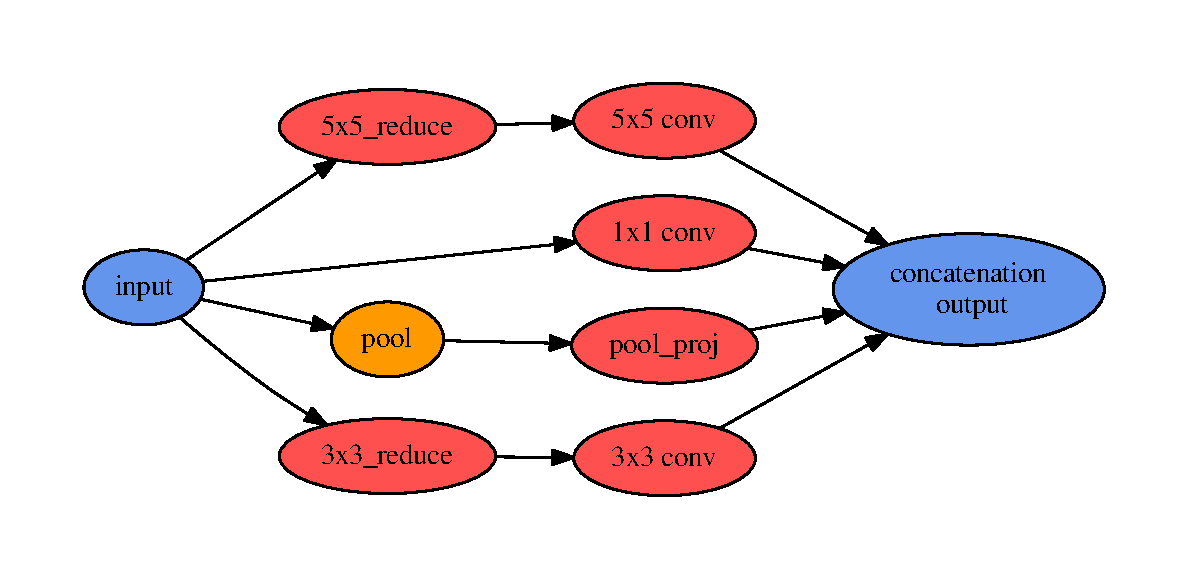
\includegraphics[scale=.45]{fig/inception.pdf}\\
  \caption{Inception Module. $n\times n$ stands for size $n$ receptive field, $n\times n\_reduce$ stands for the $1\times 1$ convolutional layer before the $n\times n$ convolution layer and $pool\_proj$ is another $1\times 1$ convolutional layer after the MAX pooling layer. The output layer concatenates all its input layers.}\label{incept}
\end{figure}

\subsection{Pre-training and Fine-tuning}
Even though Food-101 dataset contains large amount of images, it is still not sufficient to train the GoogLeNet well.
Training a deep CNN with millions of parameters with insufficient data could easily lead to horrible overfitting. But the idea of supervised pre-training on some huge image datasets could preventing this problem in certain degree. Compared to other randomly initialized strategies with certain distribution, supervised pre-training is to initialize the weights according to the model trained from a specific task. Indeed, initialization with pre-trained model has certain bias as there is no single dataset including all the invariance for natural images \cite{agrawal2014analyzing}, but this bias can be reduced as the pre-trained image dataset increases and the fine-tuning should be benefit from it.

We use the AlexNet, another architecture of deep CNN, as the baseline to illustrate the property of GoogLeNet.
We conduct several experiments on both architectures and use different training initialization strategies for Food-101 datasets. The scratch models are initialized with Gaussian distribution for AlexNet and Xavier algorithm for GoogLeNet%, which automatically determines the scale of initialization based on the number of input and output neurons
 \cite{glorot2010understanding}. These two initializations are used for training the original models for the ImageNet task. The ft-last and fine-tuned models are initialized with the weights pre-trained from ImageNet dataset. For the ft-last model, we just re-train the fully connected layers while the whole network is fine-tuned for the fine-tune model.
% Table generated by Excel2LaTeX from sheet 'Sheet1'
\begin{table}[htbp]
  \centering
  \caption{Top-5 Accuracy for different deep CNN architectures}
    \begin{tabular}{r|ccc}
    \toprule
          & Fine-tune & Ft-last & Scratch \\
    \midrule
    GoogLeNet & \textbf{93.51} & 82.84 & 90.45 \\
    AlexNet & \textbf{88.12} & 78.18 & 76.49 \\
    \bottomrule
    \end{tabular}%
  \label{tab:ft}%
\end{table}%



% Table generated by Excel2LaTeX from sheet 'Sheet1'
\begin{table*}[htbp]
  \centering
  \caption{Top-1 accuracy compared to other methods on Food-101 dataset in percent}
    \begin{tabular}{c|C{3cm}C{3cm}cc}
    \toprule
          & RFDC\cite{bossard14} & MLDS($\approx$\cite{singh2012unsupervised}) & GoogLeNet & AlexNet \\
    \midrule
    Top1 accuracy & 50.76 & 42.63& \textbf{78.11 }& 66.40 \\
    \bottomrule
    \end{tabular}%
    \label{tab:101}
\end{table*}%
\begin{figure*}[htbp]
  \centering
  % Requires \usepackage{graphicx}
  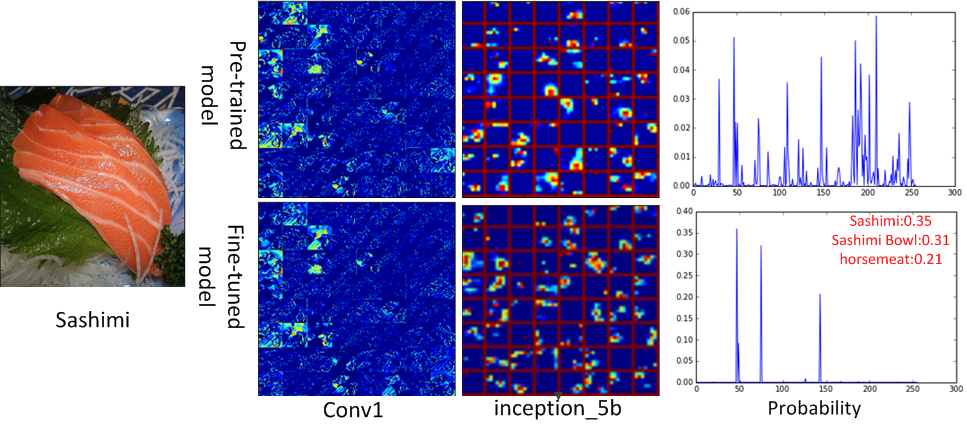
\includegraphics[scale=0.5]{fig/sashimi.png}\\
  \caption{Visualization of some feature maps of different GoogLeNet models in different layers for the same input image. 64 feature maps of each layer are shown. Conv1 is the first convolutional layer and Inception\_5b is the last convolutional layer. }
   \label{fig:sashimi}
\end{figure*}
From Table \ref{tab:ft} we can see that fine-tuning the whole network can improve the performance of the CNN for our task. Compared to other traditional computer vision methods (see Table \ref{tab:101}), GoogLeNet outperforms the other methods with large margins and we provide the state-of-the-art performance on this datasets. In Section \ref{sec:da}, the feature representations extracted from fine-tuned model are used as the input for our online domain adaptation method.

\subsection{Discussion of the unique architecture of GoogLeNet}
In the last part, we show the state-of-the-art performance for GoogLeNet on Food-101 dataset. Since few work has been found to discuss the architecture of GoogLeNet, we would like to show some interesting findings from our empirical study.

Instead of training a classifier for image recognition with deep CNN, we utilize deep CNN as the feature extractor for our adaptation task. Indeed, the classifier can take great advantage of discriminative feature representations for different categories. From our empirical study, we find that benefitting from the the unique architecture of Inception module in GoogLeNet, GoogLeNet can learn the feature representations in a efficient way while other architectures may suffer from vanished gradient a lot.

In Figure \ref{fig:sashimi} we visualize the feature maps of the pre-trained GoogLeNet model and fined-tuned GoogLeNet model with the same input image for some layers. We can see that the feature maps of the lower layer are similar as the lower level features are similar for most recognition tasks.
Then we can see that the feature maps in the high-level are different which leads to totally different recognition results.
Since only the last layer (auxiliary classifier) of the ft-last model is optimized, we can infer that the higher level features are more important which is consistent with our intuition. Also from Table \ref{tab:ft}, it is interesting to see that even though Food-101 is a relative large dataset with 1000 examples per category, the model can still takes advantage of the initialization from ImageNet dataset. 

From Table \ref{tab:ft} we can see that GoogLeNet always performances better than AlexNet on both datasets. This implies that the higher level features of GoogLeNet are more discriminative compared to AlexNet and this is due to the special architecture of its basic unit, Inception module. Table \ref{tab:cosg} and \ref{tab:cosa} show the weights' cosine similarity of each layer between the fine-tuned models and their pre-trained models. From the results we can see that the weights in the low layer are more similar which implies that these two architectures can learn the hierarchical features. As the low level features are similar for most of the tasks, the difference of the objects is determined by high-level ones which are the combination of these low level features. Also from Table \ref{tab:cosa}, we can observe that, the weights of the pre-trained and fine-tuned models are extremely similar in AlexNet . This indicates that even though ReLUs are used in both architectures, deep CNN could still suffer from vanished gradient. However, from Table \ref{tab:cosg} we can see that, fined-tuned GoogLeNet seems suffer less from this problem.
Rectified activation function is mathematically given by:
      \begin{equation}\label{relu}
        h = \max ({w^T}x,0) = \left\{ {\begin{array}{*{20}{c}}
{{w^T}x}&{{w^T}x > 0}\\
0&{else}
\end{array}} \right.
      \end{equation}

    The ReLU is inactivated when its input is below 0 and its partial derivative is 0 as well. Sparsity can improve the performance of the linear classifier on top, but on the other hand, sparse representations make the network more difficult to train as well as fine-tune. The derivative of the filter is $\frac{{\partial J}}{{\partial w}} = \frac{{\partial J}}{{\partial y}}\frac{{\partial y}}{{\partial w}} = \frac{{\partial J}}{{\partial y}}*x$ where $\frac{{\partial J}}{{\partial y}}$ denotes the partial derivative of the activation function, $y=w^Tx$ and $x$ denotes the inputs of the layer. The sparse input could lead to sparse filter derivative for back propagation which would eventually prevent the errors passing down effectively. Therefore, the filters of the fine-tuned AlexNet is extremely similar. Compared to large receptive field used in AlexNet, the inception module in GoogLeNet employs 2 additional $n\times n\_reduced$ convolutional layers before the $3\times 3$ and $5\times 5$ convolutional layers (see Figure \ref{incept}). Even though the original purpose of these two $1\times 1$ convolutional layer is for computational efficiency, these 2 convolutional layers tend to squeeze their sparse inputs and generate a dense outputs for the following layer. We can see from Table \ref{tab:sparse} that the sparsity of the $n\times n\_reduce$ layers are denser than other layers within the inception module. This makes the filters in the following layer more easily to be trained for transfer learning and generate efficient sparse representations.


\begin{table*}[htbp]
  \centering
  \caption{Cosine similarity of the layers in inception modules between fine-tuned models and pre-trained model for GoogLeNet}
    \begin{tabular}{r|cccccc}
    \toprule
    \multicolumn{7}{c}{food101} \\ \midrule
          & \multicolumn{1}{l}{1x1 } & \multicolumn{1}{l}{3x3\_reduce} & \multicolumn{1}{l}{3x3} & \multicolumn{1}{l}{5x5\_reduce} & \multicolumn{1}{l}{5x5} & \multicolumn{1}{l}{pool\_proj } \\
    inception\_3a & 0.71  & 0.72  & 0.63  & 0.67  & 0.73  & 0.68 \\
    inception\_3b & 0.56  & 0.63  & 0.50  & 0.71  & 0.60  & 0.53 \\
    inception\_4a & 0.43  & 0.50  & 0.50  & 0.47  & 0.62  & 0.36 \\
    inception\_4b & 0.48  & 0.52  & 0.57  & 0.50  & 0.67  & 0.35 \\
    inception\_4c & 0.57  & 0.61  & 0.59  & 0.53  & 0.63  & 0.47 \\
    inception\_4d & 0.54  & 0.58  & 0.53  & 0.54  & 0.64  & 0.44 \\
    inception\_4e & 0.53  & 0.54  & 0.61  & 0.55  & 0.62  & 0.42 \\
    inception\_5a & 0.43  & 0.47  & 0.53  & 0.45  & 0.57  & 0.34 \\
    inception\_5b & 0.36  & 0.39  & 0.46  & 0.38  & 0.52  & 0.37 \\
    \bottomrule
    \end{tabular}%
  \label{tab:cosg}%
\end{table*}%


\begin{table*}[htbp]
  \centering
  \caption{Cosine similarity of the layers between fine-tuned models and pre-trained model for AlexNet}
    \begin{tabular}{r|ccccccc}
    \toprule
          & conv1 & conv2 & conv3 & conv4 & conv5 & fc6   & fc7 \\
    \midrule
    food101 & 0.996 & 0.984 & 0.963 & 0.960 & 0.963 & 0.925 & 0.933 \\
    \bottomrule
    \end{tabular}%
  \label{tab:cosa}%
\end{table*}%

% Table generated by Excel2LaTeX from sheet 'google'
\begin{table*}[htbp]
  \centering
  \caption{Sparsity of the output for each unit in GoogLeNet inception module for training data from Food101 in percent}
    \begin{tabular}{r|cccccc}
    \toprule
          & 1x1  & 3x3\_reduce & 3x3  & 5x5\_reduce & 5x5  & pool\_proj  \\
    \midrule
    inception\_3a & $69.3\pm 1.3$  & $69.6 \pm 1.1$  & $80.0\pm  1.0$& $64.1\pm  2.2$& $75.8\pm  1.6$& $76.2\pm 5.4$\\
    inception\_3b & $92.8 \pm 0.9$&$ 76.5 \pm 0.9$& $94.7\pm 0.9 $&$ 71.6 \pm 2.3 $&$ 94.4\pm 0.5 $&$ 94.7 \pm 1.6$\\
    inception\_4a & $90.9 \pm 0.9$& $70.0\pm 1.2 $& $93.8\pm 1.1 $& $63.3\pm 4.0 $& $91.9\pm 1.8 $& $95.1\pm 2.0$\\
    inception\_4b & $71.9 \pm 1.6$& $67.5\pm 1.2$ & $75.4\pm  1.0$& $58.5 \pm 2.6$& $78.9\pm  1.6$& $85.6\pm 3.6$\\
    inception\_4c & $75.1 \pm 2.4$& $72.6 \pm 1.3$& $81.0\pm 2.0$ & $66.3\pm 6.1 $& $79.7 \pm 3.6$& $88.1\pm 3.3$\\
    inception\_4d & $87.3 \pm 2.7$& $78.0 \pm 2.2$& $88.0\pm 1.6$& $67.9\pm 3.1 $& $88.9\pm 2.8 $& $93.0\pm 2.2$\\
    inception\_4e & $91.8\pm  1.1$& $62.3\pm 2.2 $& $91.0\pm 2.5 $& $49.5 \pm 3.7$& $94.0 \pm 1.0$& $92.3\pm 1.5$\\
    inception\_5a & $78.7 \pm 1.6$& $66.5\pm  1.7$& $82.3\pm 2.6 $& $59.9\pm 3.2 $& $86.4\pm 2.3 $& $87.1\pm 2.6$\\
    inception\_5b & $88.2\pm 2.3 $& $86.8 \pm 1.6$&$ 83.3\pm 4.4$ & $84.0\pm 3.1 $& $81.4\pm 5.3$  & $94.7\pm 1.5$\\
    \bottomrule
    \end{tabular}%
  \label{tab:sparse}%
\end{table*}%

The unique structure of the Inception module guarantees that the sparse outputs from previous layer can be squeezed with the $1\times 1$ convolutional layers and feed to convolutional layers with bigger receptive field to generate sparser representation. The squeeze action promises the back propagation error can be transferred more efficiently and makes the whole network more flexible to fit different recognition tasks.

